\subsection{Descripci\'on}
Tenemos como datos de entrada una lista de n cursos, cada uno de los cuales posee un par de enteros, el primero indica el comienzo del mismo y el segundo el fin, con inicio menor igual que fin. \\
Y debemos organizarlos de tal manera de lograr disponer la máxima cantidad de cursos posibles, sin que se solapen entre sí. Dos cursos c1 (i1,f1) y c2 (i2,f2) no se solapan entre ellos, si i1 $\leq$ f1 <  i2  ó f1 $\geq$ i1 > f2.

A continuación se muestra un ejemplo y una posible solución.\\

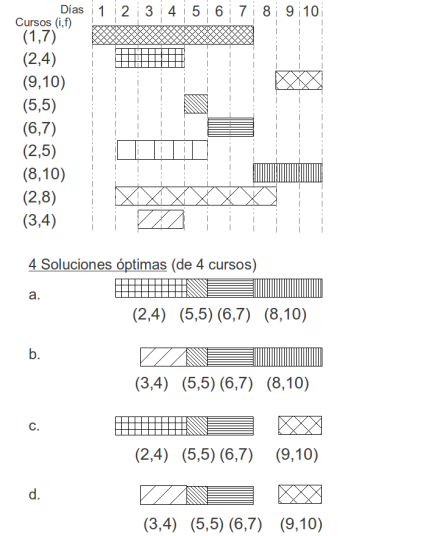
\includegraphics[scale=1]{ej2/Graficos/ej2a400x480.png} \\

Notar que pueden existir varias soluciones óptimas, y el algoritmo debe dar una de ellas sin ninguna otra especificación. Si todos los cursos se solapan entre sí, la solución sería tomar uno cualquiera.\\
